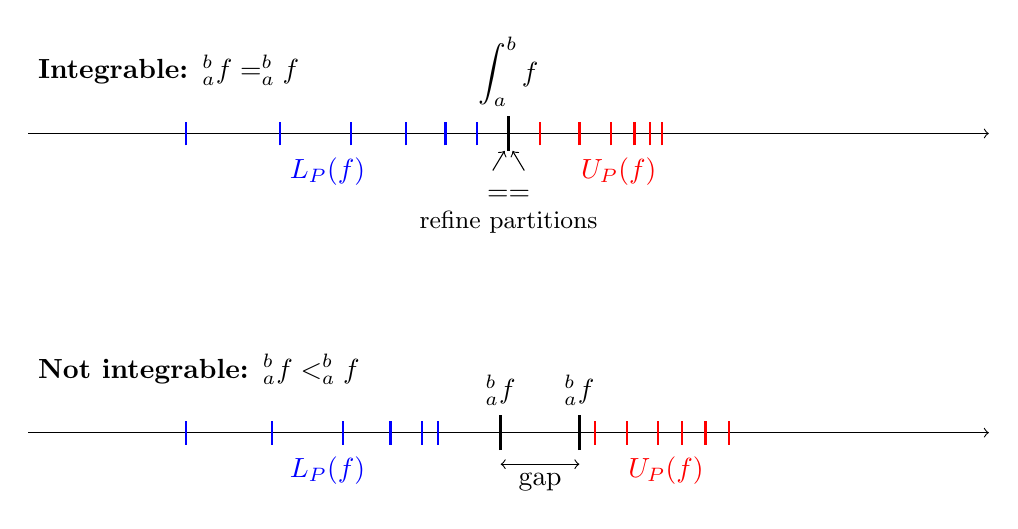
\begin{tikzpicture}[x=1cm,y=1cm]
  % Two number lines: integrable (meeting) vs non-integrable (gap)

  % ---------------- Integrable ----------------
  \node[anchor=west,font=\bfseries] at (0,5.4) {Integrable: $\lowint_a^b f = \upint_a^b f$};
  \draw[->] (0,4.6) -- (12.2,4.6);

  % Lower sums (left cluster) — blue
  \foreach \x in {2.0,3.2,4.1,4.8,5.3,5.7} {
    \draw[blue,thick] (\x,4.45) -- (\x,4.75);
  }
  \node[below,blue] at (3.8,4.42) {$L_P(f)$};

  % Upper sums (right cluster) — red
  \foreach \x in {6.5,7.0,7.4,7.7,7.9,8.05} {
    \draw[red,thick] (\x,4.45) -- (\x,4.75);
  }
  \node[below,red] at (7.5,4.42) {$U_P(f)$};

  % Common value — prominent black line
  \draw[very thick] (6.1,4.38) -- (6.1,4.82);
  \node[above] at (6.1,4.82) {$\displaystyle\int_a^b f$};

  \draw[->,thin] (5.9,4.13) -- (6.05,4.38);
  \draw[->,thin] (6.3,4.13) -- (6.15,4.38);
  \node[below,align=center] at (6.1,4.0) {$=\lowint=\upint$\\[-2pt]{\small refine partitions}};

  % ---------------- Not integrable ----------------
  \node[anchor=west,font=\bfseries] at (0,1.6) {Not integrable: $\lowint_a^b f < \upint_a^b f$};
  \draw[->] (0,0.8) -- (12.2,0.8);

  % Lower sums (left cluster) — blue
  \foreach \x in {2.0,3.1,4.0,4.6,5.0,5.2} {
    \draw[blue,thick] (\x,0.65) -- (\x,0.95);
  }
  \node[below,blue] at (3.8,0.62) {$L_P(f)$};

  % Upper sums (right cluster) — red
  \foreach \x in {7.2,7.6,8.0,8.3,8.6,8.9} {
    \draw[red,thick] (\x,0.65) -- (\x,0.95);
  }
  \node[below,red] at (8.1,0.62) {$U_P(f)$};

  % Lower & upper integrals as barrier points
  \draw[very thick] (6.0,0.58) -- (6.0,1.02);
  \draw[very thick] (7.0,0.58) -- (7.0,1.02);
  \node[above] at (6.0,1.02) {$\lowint_a^b f$};
  \node[above] at (7.0,1.02) {$\upint_a^b f$};

  \draw[<->] (6.0,0.4) -- (7.0,0.4);
  \node[below] at (6.5,0.4) {gap};
\end{tikzpicture}
